Da ein Grossteil dieses Versuch in der korrekten Justierung und Durchf\"uhrung
besteht, ist dieses Kapitel etwas umfangreicher als \"ublich.

% ---------------------------------------------------------------------------- $
\subsection{Versuchsanordnung}
\label{subsec:versuchsanordnung}
% ---------------------------------------------------------------------------- $

\begin{figure}[h!t]
    \centering
    \resizebox{\textwidth}{!}{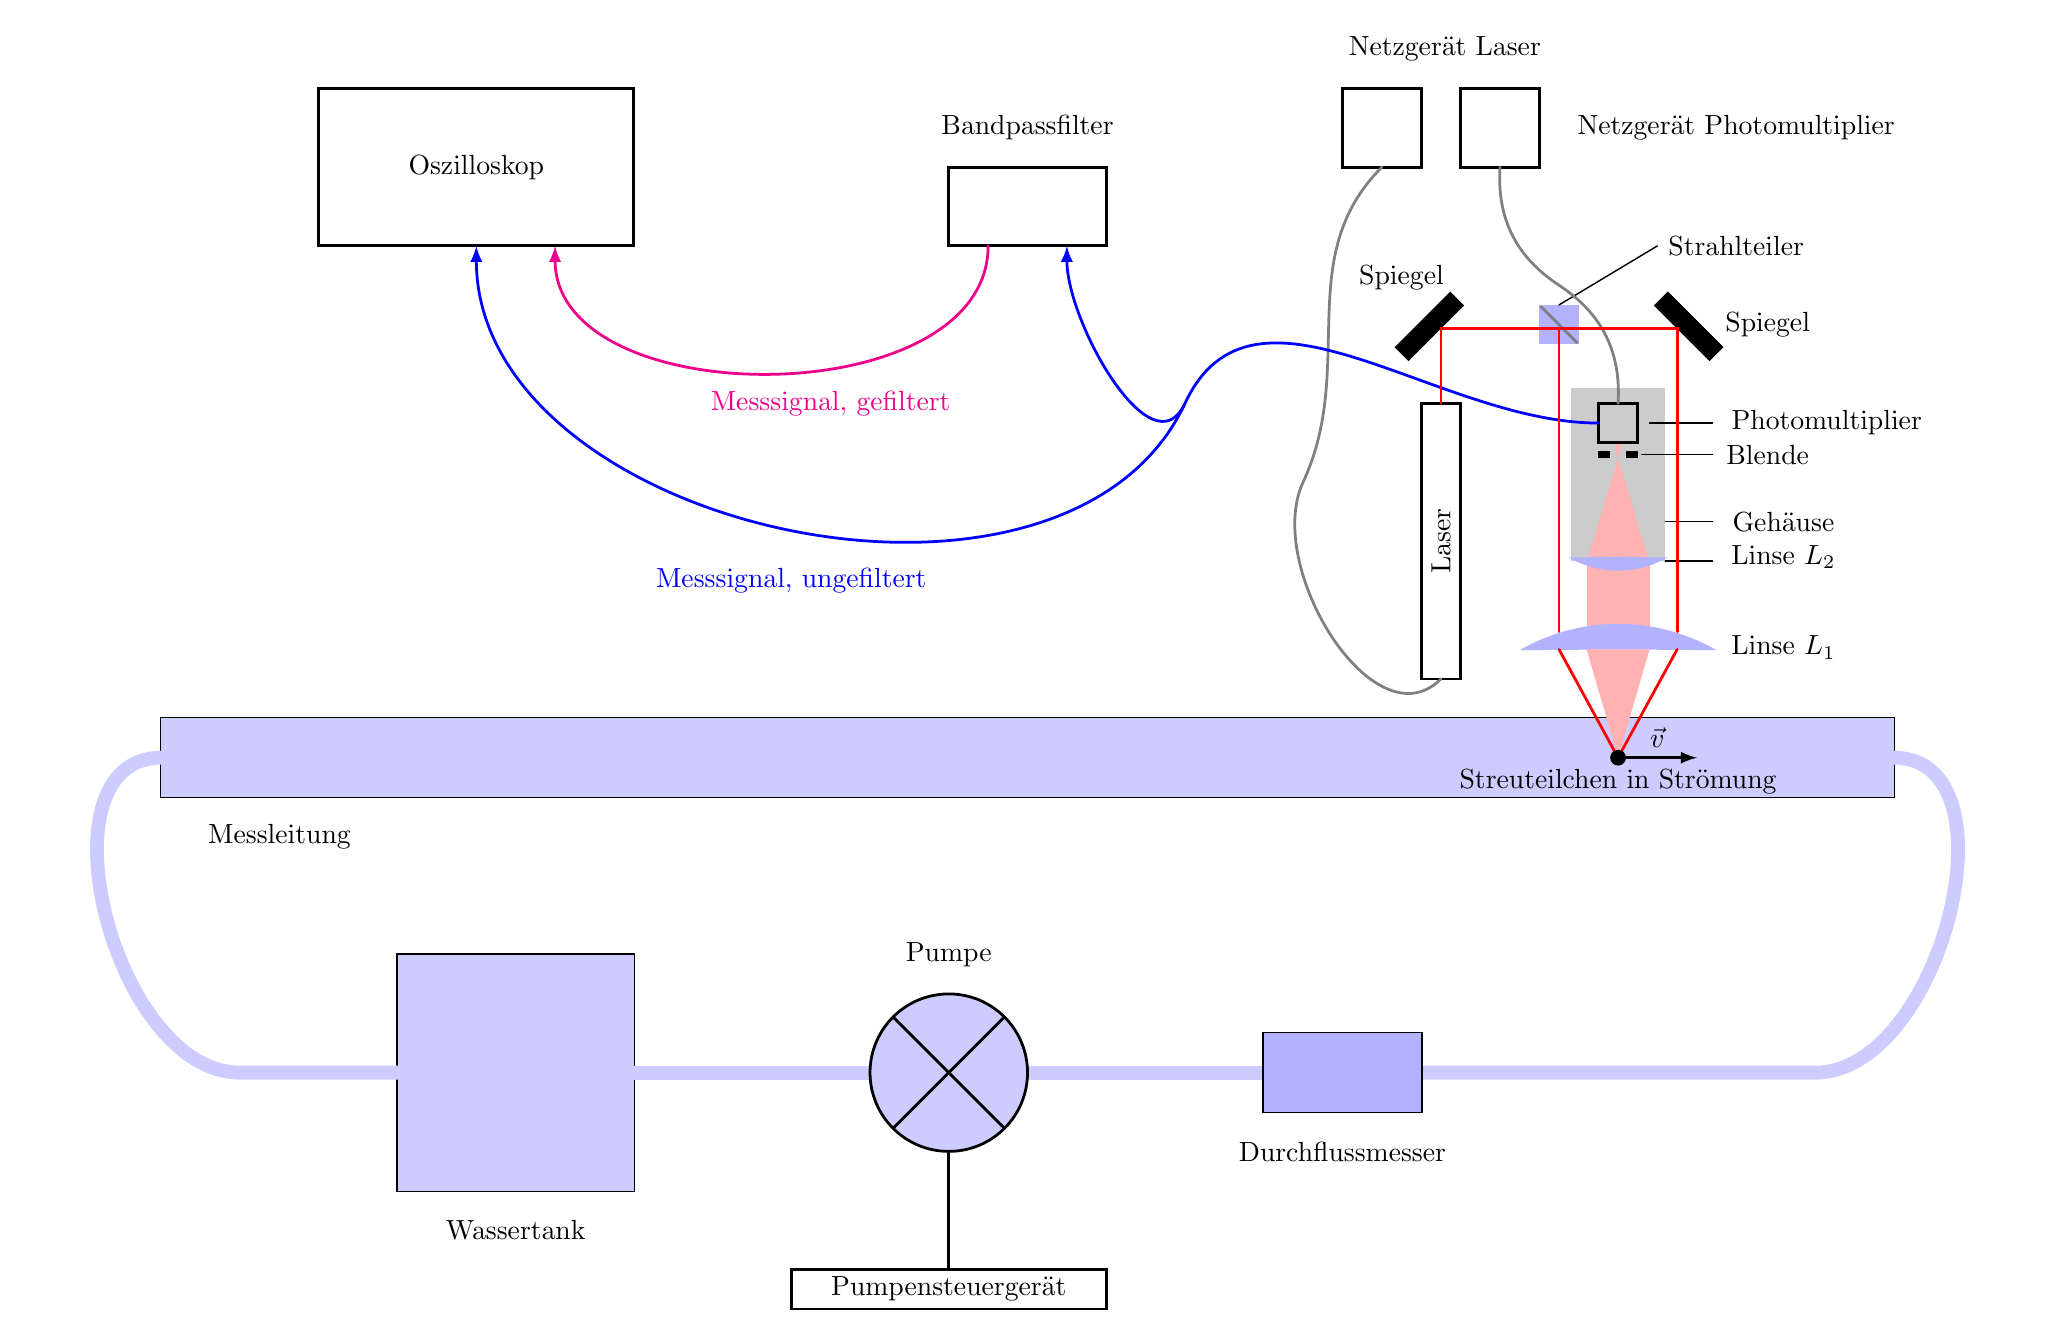
\begin{tikzpicture}
    \begin{scope}[x={(0mm,300mm)},y={(0mm,185mm)},line width=1pt,cap=round]
        % bounding box
        %\draw[black] (25mm,0mm) rectangle (275mm,175mm);

        % oscilloscope
        \draw[black] (60mm,160mm) rectangle (100mm,140mm);
        \node at (80mm,150mm) {Oszilloskop};

        % filter
        \draw[black] (140mm,150mm) rectangle (160mm,140mm);
        \node at (150mm,155mm) {Bandpassfilter};

        % PSU laser
        \draw[black] (190mm,160mm) rectangle (200mm,150mm);
        \node at (203mm,165mm) {Netzger\"at Laser};

        % PSU photomultiplier
        \draw[black] (205mm,160mm) rectangle (215mm,150mm);
        \node at (240mm,155mm) {Netzger\"at Photomultiplier};

        % measurement pipe
        \draw[black] (40mm,70mm) rectangle (260mm,80mm);
        \fill[blue!20] (40mm,70mm) rectangle (260mm,80mm);
        \node at (55mm,65mm) {Messleitung};

        % water tank
        \draw[black]   (70mm,20mm) rectangle (100mm,50mm);
        \fill[blue!20] (70mm,20mm) rectangle (100mm,50mm);
        \node at (85mm,15mm) {Wassertank};

        % pipe to tank
        \draw[-,blue!20,line width=5pt] (40mm,75mm)
            to [out=180,in=180] (50mm,35mm)
            to [out=0,in=180] (70mm,35mm);
        % tank to pump
        \draw[-,blue!20,line width=5pt] (100mm,35mm)
            to [out=180,in=180] (130mm,35mm);
        % pump to flow sensor
        \draw[-,blue!20,line width=5pt] (150mm,35mm)
            to (180mm,35mm);
        % flow sensor to pipe
        \draw[-,blue!20,line width=5pt] (200mm,35mm)
            to [out=0,in=180] (250mm,35mm)
            to [out=0,in=0] (260mm,75mm);

        % pump
        \fill[blue!20] (140mm,35mm) circle(10mm);
        \draw[black]   (140mm,35mm) circle(10mm);
        \draw[black,rotate around={-45:(140mm,35mm)}] (130mm,35mm) -- (150mm,35mm);
        \draw[black,rotate around={+45:(140mm,35mm)}] (130mm,35mm) -- (150mm,35mm);
        \node at (140mm,50mm) {Pumpe};

        % pump controller
        \draw[black] (140mm,25mm) -- (140mm,10mm);
        \draw[black]   (120mm,5mm) rectangle (160mm,10mm);
        \node at (140mm,7.5mm) {Pumpensteuerger\"at};


        % flow sensor
        \draw (180mm,30mm) rectangle (200mm,40mm);
        \fill[blue!30] (180mm,30mm) rectangle (200mm,40mm);
        \node at (190mm,25mm) {Durchflussmesser};

        % laser and cable
        \draw[black] (200mm,120mm) rectangle (205mm,85mm);
        \draw[black!50]        (195mm,150mm)
            to [out=-135,in=65] (185mm,110mm)
            to [out=-115,in=-135] (202.5mm,85mm);
        \node[rotate=90] at (202.5mm,102.5mm) {Laser};

        % mirror 1
        \fill[black,rotate around={45:(197.5mm,126.25mm)}] (197.5mm,125mm) rectangle (207.5mm,127.5mm);
        \node at (197.5mm,136mm) {Spiegel};

        % beam splitter
        \fill[blue!30]  (215mm,127.5mm) rectangle (220mm,132.5mm);
        \draw[black!50] (215.2mm,132.3mm) -- (219.8mm,127.7mm);
        \draw[black,line width=0.5pt] (217.5mm,132.5mm) -- (230mm,140mm);
        \node at (240mm,140mm) {Strahlteiler};

        % mirror 2
        \fill[black,rotate around={-45:(237.5mm,126.25mm)}] (227.5mm,125mm) rectangle (237.5mm,127.5mm);
        \node at (244mm,130mm) {Spiegel};

        % housing around detector and L2
        \fill[black!20] (219mm,122mm) rectangle (231mm,100mm);
        \draw[black,line width=0.5pt] (231mm,105mm) -- (237mm,105mm);
        \node at (246mm,105mm) {Geh\"ause};


        % dispersed light below lenses
        \fill[red!30] (221mm,90mm) rectangle (229mm,99.75mm);
        \fill[red!30] (221mm,99.75mm) -- (225mm,113mm) -- (229mm,99.75mm);
        \fill[red!30] (225mm,113mm) -- (224.5mm,115mm) -- (225.5mm,115mm);

        % detector and power cable and signal cables
        \draw[black] (222.5mm,120mm) rectangle (227.5mm,115mm);
        \draw[black!50] (210mm,150mm) to [bend right] (217.5mm,135mm) to [bend left] (225mm,120mm);
        \draw[-latex,blue] (222.5mm,117.5mm)
            to [out=180,in=65] (170mm,120mm)
            to [out=-115,in=-90] (155mm,140mm);
        \draw[-latex,blue] (170mm,120mm)
            to [out=-115,in=-90] (80mm,140mm);
        \draw[-latex,magenta] (145mm,140mm)
            to [out=-90,in=-90] (90mm,140mm);
        \node[magenta] at (125mm,120mm) {Messsignal, gefiltert};
        \node[blue] at (120mm,97.5mm) {Messsignal, ungefiltert};
        \node at (251.5mm,117.5mm) {Photomultiplier};
        \draw[black,line width=0.5pt] (229mm,117.5mm) -- (237mm,117.5mm);

        % aperture
        \fill[black] (222.5mm,114mm) rectangle (224mm,113mm);
        \fill[black] (226mm,114mm) rectangle (227.5mm,113mm);
        \draw[black,line width=0.5pt] (228mm,113.5mm) -- (237mm,113.5mm);
        \node at (244mm,113.5mm) {Blende};

        % lens L2
        \fill[blue!30] (225.25mm,100.5mm) -- (225mm,98.75mm) arc[start angle=-90,delta angle=-30,radius=12.5mm]  -- cycle;
        \fill[blue!30] (224.75mm,100.5mm) -- (225mm,98.75mm) arc[start angle=-90,delta angle=30,radius=12.5mm] -- cycle;
        \draw[black,line width=0.5pt] (231mm,100mm) -- (237mm,100mm);
        \node at (246mm,100.5mm) {Linse $L_2$};

        % lens L1
        \fill[blue!30] (224.75mm,88.75mm) -- (225mm,92mm) arc[start angle=90,delta angle=-30,radius=25mm] -- cycle;
        \fill[blue!30] (225.25mm,88.75mm) -- (225mm,92mm) arc[start angle=90,delta angle=30,radius=25mm]  -- cycle;
        \node at (246mm,89mm) {Linse $L_1$};

        % Laser beams
        % laser -> L1
        \draw[red] (202.5mm,120mm) -- (202.5mm,129.5mm) -- (217.5mm,129.5mm) -- (217.5mm,91mm);
        % L1 -> L1
        \draw[red] (217.5mm,88.75mm) -- (225mm,75mm) -- (232.5mm,88.75mm);
        % L1 -> beam splitter
        \draw[red] (232.5mm,91mm) -- (232.5mm,129.5mm) -- (217.5mm,129.5mm);
        % particle -> L1 (dispersion)
        \fill[red!30] (225mm,75mm) -- (229mm,88.75mm) -- (221mm,88.75mm);

        % particle
        \fill[black] (225mm,75mm) circle(1mm);
        \draw[-latex] (225mm,75mm) -- (235mm,75mm);
        \node at (230mm,77.5mm) {$\vec{v}$};
        \node at (225mm,72mm) {Streuteilchen in Str\"omung};

    \end{scope}
\end{tikzpicture}
}
    \caption{%
        Versuchsanordnung, schematisch
    }
    \label{fig:versuchsanordnung:schema}
\end{figure}

\begin{figure}[h!t]
    \centering
    \resizebox{.67\textwidth}{!}{\begin{tikzpicture}
    \begin{scope}[x={(0mm,300mm)},y={(0mm,199mm)},line width=1pt,cap=round]
        \node[anchor=south west,inner sep=0mm] at (0mm,0mm) {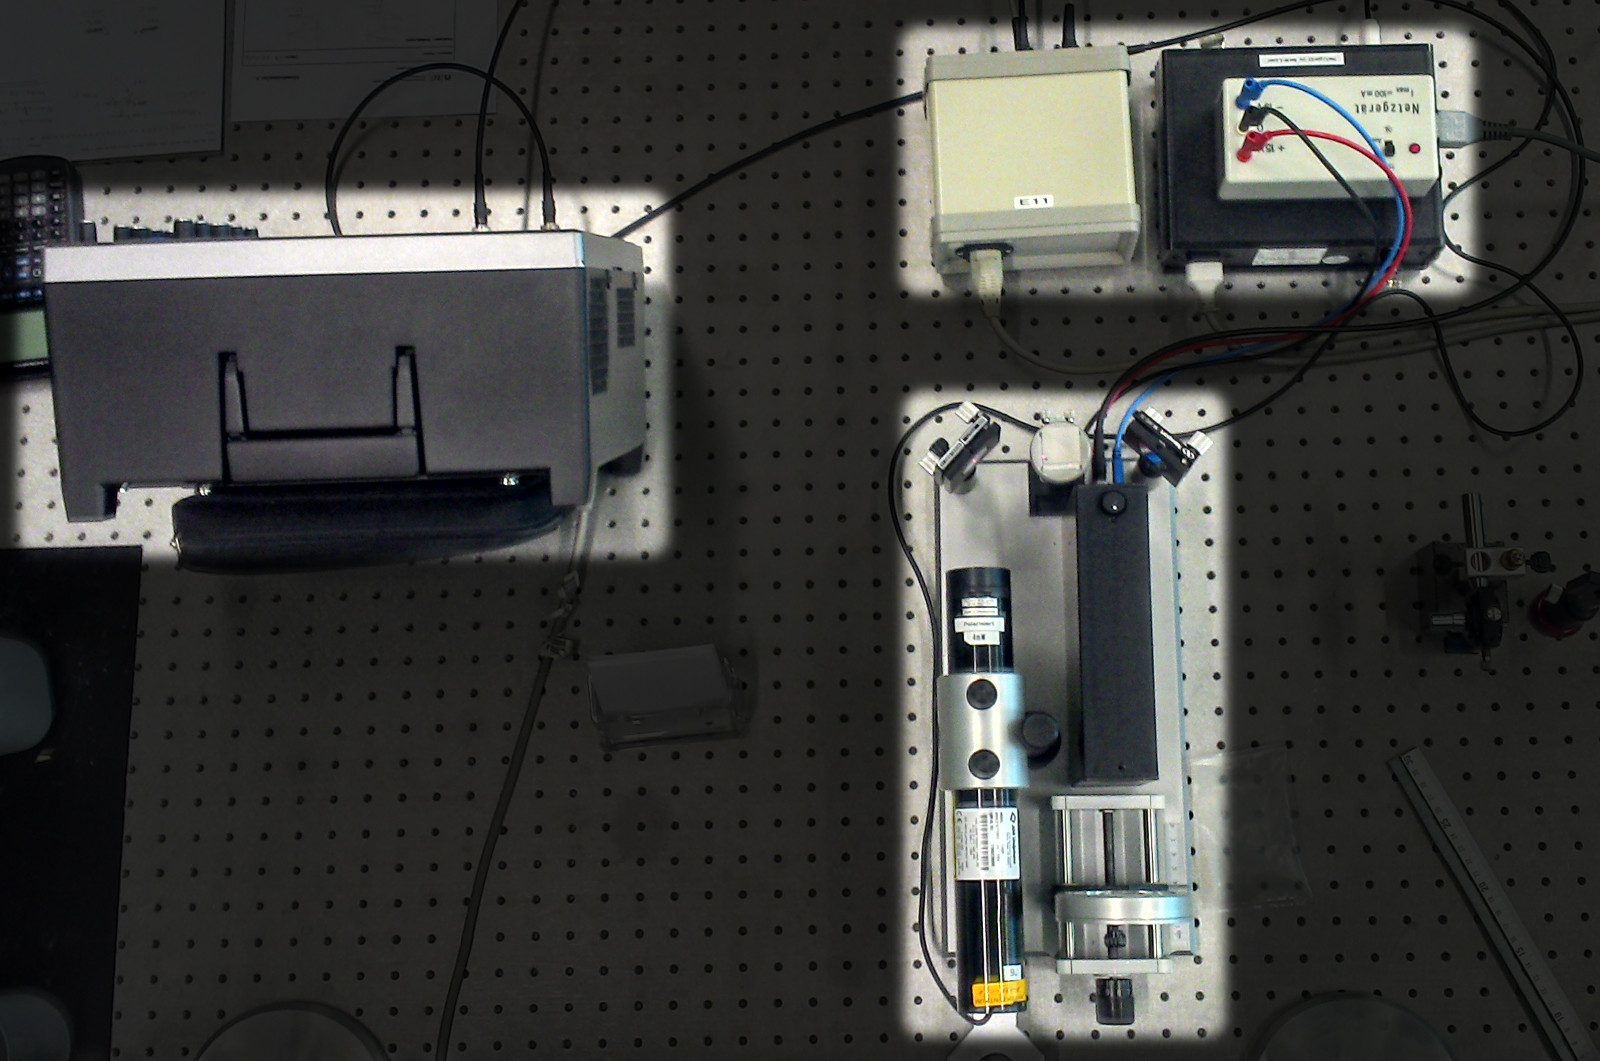
\includegraphics[width=300mm]{images/versuchsanordnung.jpeg}};

        % bounding box
        \draw[green] (0mm,0mm) rectangle (300mm,199mm);

        \node[white] at (40mm,140mm) {\Large{Oszilloskop}};

        \node[white] at (160mm,50mm) {\Large{Laser}};

        \node[white] at (160mm,120mm) {\Large{Spiegel}};

        \draw[cyan] (225mm,30mm) -- (234mm,30mm);
        \node[white] at (245mm,30mm) {\Large{Linse $L_1$}};

        \draw[cyan] (210mm,80mm) -- (234mm,80mm);
        \node[white] at (250mm,80mm) {\Large{\parbox{30mm}{\raggedright Geh\"ause mit \\Photomultiplier,\\ Blende und Linse $L_2$}}};

        \draw[cyan] (225mm,120mm) -- (234mm,120mm);
        \node[white] at (245mm,120mm) {\Large{Spiegel}};

        \node[black] at (195mm,175mm) {\Large{Bandpassfilter}};

        \node[white] at (235mm,157.5mm) {\Large{Netzger\"ate}};
    \end{scope}
\end{tikzpicture}
}
    \caption{%
        Versuchsanordnung, Vogelperspektive. Anordnung ist gr\"osstenteils mit
        dem Schema aus Abbildung \ref{fig:versuchsanordnung:schema} identisch.
    }
    \label{fig:versuchsanordnung:birdseye}
\end{figure}

\begin{figure}[h!t]
    \centering
    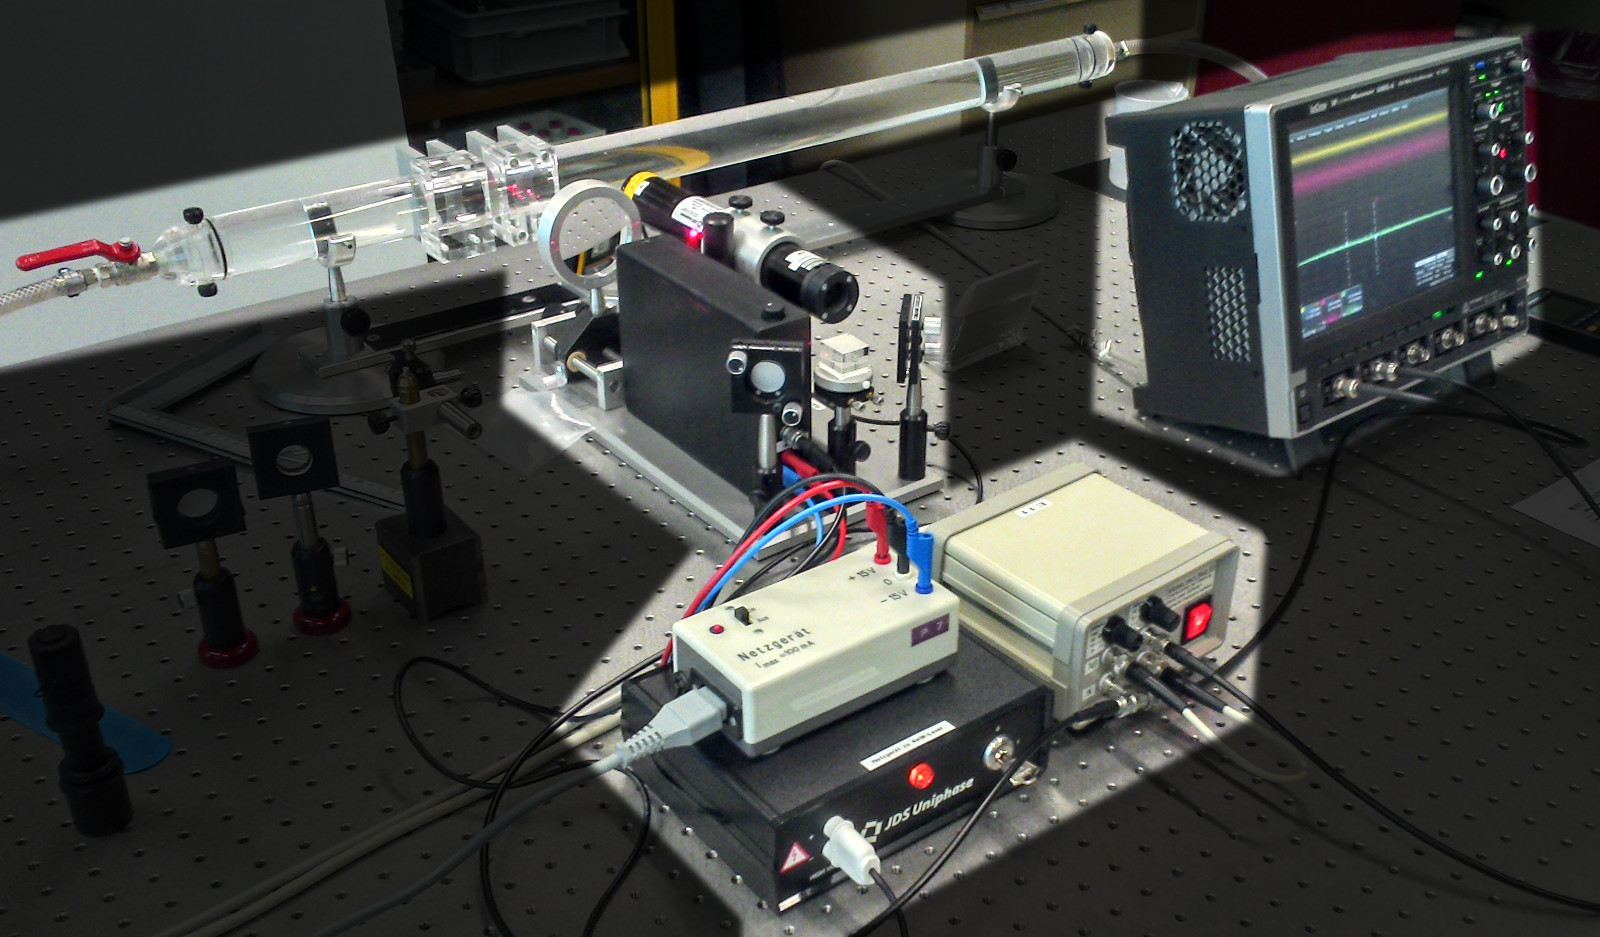
\includegraphics[width=.67\textwidth]{images/versuchsanordnung2.jpeg}
    \caption{%
        Versuchsanordnung,   andere   Perspektive. Messleitung   Sichtbar   im
        Hintergrund.
    }
    \label{fig:versuchsanordnung:perspective}
\end{figure}

Grunds\"atzlich  folgt   der  Versuchsaufbau  den  in   den  Arbeitsgrundlagen
beschriebenen    Angaben. Die   gesamte    Anordnung   ist    schematisch   in
Abbildung     \ref{fig:versuchsanordnung:schema}    dargestellt,     Abbildung
\ref{fig:versuchsanordnung:birdseye}  ist   die  entsprechende  fotographische
Dokumentation.  Abbildung  \ref{fig:versuchsanordnung:perspective} zeigt einen
anderen Blickwinkel auf die Apparaturen.

Um \"Uberlastung  durch Umgebungslicht zu verhindern,  ist der Photomultiplier
zusammen mit der Blende und der Linse $L_2$ in einem Geh\"ause eingelassen. Um
die Blende einzustellen und die Lage der Laserstrahlen zu \"uberpr\"ufen, kann
dieses  abgenommen  werden,  es  sollte aber  bei  Aktivierung  des  Detektors
montiert sein. Der Detektor  wird zwar nicht sofort zerst\"ort,  falls er ohne
Geh\"ause  eingeschaltet  wird,  der  Vorgang ist  aber  der  Lebensdauer  des
Ger\"ats nicht zutr\"aglich.

Das Geh\"ause kann in den Abbildungen \ref{fig:versuchsanordnung:birdseye} und
\ref{fig:versuchsanordnung:perspective} gesehen werden.


% ---------------------------------------------------------------------------- $
\clearpage
\subsection{Messger\"ate}
\label{subsec:messgerate}
% ---------------------------------------------------------------------------- $

\begin{table}[h!t]
    \centering
    \caption{Ger\"ateliste}
    \begin{tabular}{ll}
        \toprule
        \textsc{Ger\"at}
        & \textsc{Typ}
        \\

        \midrule

        Oszilloskop
        & LeCroy WaveRunner 64MXi-A
        \\

        Laser
        & JDS Uniphase 1122P, \SI{4}{\milli\watt}, polarisiert, $\lambda = \SI{632,8}{\nano\meter}$
        \\

        Pumpe
        & %TODO
        \\

        Durchflussmesser
        & %TODO
        \\

        Detektor
        & Hamamatsu H9656-02 Photomultiplier
        \\

        Linse $L_1$
        & %TODO
        \\

        Linse $L_2$
        & \\

        Messleitung
        & Plexiglasrohr, Innendurchmesser \SI{40 \pm 0.5}{\milli\meter}
        \\

        Bandpassfilter
        & Tiefpass: \SI{3}{\kilo\hertz} bis \SI{300}{\kilo\hertz}, Hochpass: \SI{0.3}{\kilo\hertz} bis \SI{30}{\kilo\hertz}
        \\

        \bottomrule
    \end{tabular}
\end{table}


% ---------------------------------------------------------------------------- $
\clearpage
\subsection{Ablauf}
\label{subsec:ablauf}
% ---------------------------------------------------------------------------- $

Wie  erw\"ahnt,  ist eine  korrekte  justierung  dieses Versuches  f\"ur  eine
erfolgreiche  Durchf\"uhrung von  grosser Wichtigkeit. Sie  beanspruchte einen
betr\"achtlichen  Teil  der  zur   Verf\"ugung  stehenden  Zeit  (beinahe  die
H\"alfte) und soll hier entsprechend auch gut dokumentiert werden.

Die Krux am Ganzen ist, dass  die Laserstrahlen sich sauber in der Messleitung
kreuzen und anschliessend korrekt in den Detektor gef\"uhrt werden.

Dazu wurden zuerst an den in Abbildung \ref{fig:justierung} mit blauen Kreuzen
markierten  Punkten die  H\"ohe  der Laserstrahlen  gemessen  und mittels  der
Spiegel (siehe auch  Abbildung \ref{fig:spiegel}) und der Linse  $L_1$ auf die
gleiche H\"ohe eingestellt (so gut als m\"oglich, dieses Verfahren alleine ist
noch nicht genau genug).

\begin{figure}[h!t]
    \centering
    \resizebox{.67\textwidth}{!}{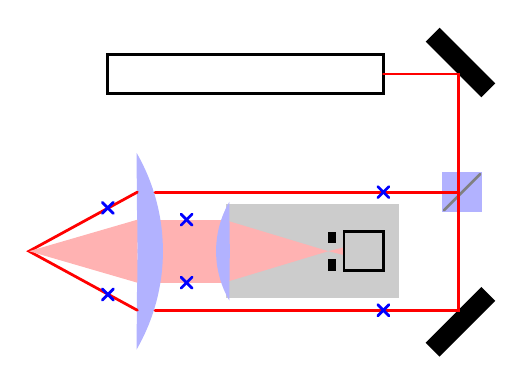
\begin{tikzpicture}
    \begin{scope}[x={(0mm,300mm)},y={(0mm,185mm)},line width=1pt,cap=round,rotate=-90]
        % bounding box
        %\draw[black] (190mm,70mm) rectangle (245mm,140mm);

        % laser and cable
        \draw[black] (200mm,120mm) rectangle (205mm,85mm);

        % mirror 1
        \fill[black,rotate around={45:(197.5mm,126.25mm)}] (197.5mm,125mm) rectangle (207.5mm,127.5mm);

        % beam splitter
        \fill[blue!30]  (215mm,127.5mm) rectangle (220mm,132.5mm);
        \draw[black!50] (215.2mm,132.3mm) -- (219.8mm,127.7mm);
        %\node at (215mm,120mm) {\footnotesize{1}};

        % mirror 2
        \fill[black,rotate around={-45:(237.5mm,126.25mm)}] (227.5mm,125mm) rectangle (237.5mm,127.5mm);

        % housing around detector and L2
        \fill[black!20] (219mm,122mm) rectangle (231mm,100mm);


        % dispersed light below lenses
        \fill[red!30] (221mm,90mm) rectangle (229mm,99.75mm);
        \fill[red!30] (221mm,99.75mm) -- (225mm,113mm) -- (229mm,99.75mm);
        \fill[red!30] (225mm,113mm) -- (224.5mm,115mm) -- (225.5mm,115mm);

        % detector and power cable and signal cables
        \draw[black] (222.5mm,120mm) rectangle (227.5mm,115mm);

        % aperture
        \fill[black] (222.5mm,114mm) rectangle (224mm,113mm);
        \fill[black] (226mm,114mm) rectangle (227.5mm,113mm);

        % lens L2
        \fill[blue!30] (225.25mm,100.5mm) -- (225mm,98.75mm) arc[start angle=-90,delta angle=-30,radius=12.5mm]  -- cycle;
        \fill[blue!30] (224.75mm,100.5mm) -- (225mm,98.75mm) arc[start angle=-90,delta angle=30,radius=12.5mm] -- cycle;

        % lens L1
        \fill[blue!30] (224.75mm,88.75mm) -- (225mm,92mm) arc[start angle=90,delta angle=-30,radius=25mm] -- cycle;
        \fill[blue!30] (225.25mm,88.75mm) -- (225mm,92mm) arc[start angle=90,delta angle=30,radius=25mm]  -- cycle;

        % Laser beams
        % laser -> L1
        \draw[red] (202.5mm,120mm) -- (202.5mm,129.5mm) -- (217.5mm,129.5mm) -- (217.5mm,91mm);
        % L1 -> L1
        \draw[red] (217.5mm,88.75mm) -- (225mm,75mm) -- (232.5mm,88.75mm);
        % L1 -> beam splitter
        \draw[red] (232.5mm,91mm) -- (232.5mm,129.5mm) -- (217.5mm,129.5mm);
        % particle -> L1 (dispersion)
        \fill[red!30] (225mm,75mm) -- (229mm,88.75mm) -- (221mm,88.75mm);

        % forward beam, left
        \draw[blue,rotate around={45:(217.5mm,120mm)}] (216.5mm,120mm) -- (218.5mm,120mm);
        \draw[blue,rotate around={-45:(217.5mm,120mm)}] (216.5mm,120mm) -- (218.5mm,120mm);

        % forward beam, right
        \draw[blue,rotate around={45:(232.5mm,120mm)}] (231.5mm,120mm) -- (233.5mm,120mm);
        \draw[blue,rotate around={-45:(232.5mm,120mm)}] (231.5mm,120mm) -- (233.5mm,120mm);

        % forward beam, after L1, left
        \draw[blue,rotate around={45:(219.5mm,85mm)}] (218.5mm,85mm) -- (220.5mm,85mm);
        \draw[blue,rotate around={-45:(219.5mm,85mm)}] (218.5mm,85mm) -- (220.5mm,85mm);

        % forward beam, after L1, right
        \draw[blue,rotate around={45:(230.5mm,85mm)}] (229.5mm,85mm) -- (231.5mm,85mm);
        \draw[blue,rotate around={-45:(230.5mm,85mm)}] (229.5mm,85mm) -- (231.5mm,85mm);

        % backwards beam, left
        \draw[blue,rotate around={45:(221mm,95mm)}] (220mm,95mm) -- (222mm,95mm);
        \draw[blue,rotate around={-45:(221mm,95mm)}] (220mm,95mm) -- (222mm,95mm);

        % backwards beam, right
        \draw[blue,rotate around={45:(229mm,95mm)}] (228mm,95mm) -- (230mm,95mm);
        \draw[blue,rotate around={-45:(229mm,95mm)}] (228mm,95mm) -- (230mm,95mm);
    \end{scope}
\end{tikzpicture}
}
    \caption{%
        Referenzpunkte f\"ur Kalibrierung (blau markiert)
    }
    \label{fig:justierung}
\end{figure}

Anschliessend wurde
%TODO: Instrument
benutzt,   um   die   beiden   Laserstrahlen   auf   eine   Wand   gegen\"uber
der   Versuchsanordnung  zu   projizieren. Dies   erm\"oglichte  eine   exakte
Zusammenf\"uhrung  der Laserstrahlen. Danach  wurde  sichergestellt, dass  die
Streuungen und Reflexionen der Strahlen,  welche zur\"uck in Richtung Detektor
gingen,  alle  auf  gleicher  H\"ohe   lagen,  indem  H\"ohe  und  Winkel  der
Messleitung korrekt eingestellt wurden. Abbildung \ref{fig:lensL1} zeigt diese
Strahlen vor ihrer Justierung.

Letzlich wurde \"uberpr\"uft, dass  der Kreuzungspunkt der gestreuten Strahlen
genau in der Blende (sichtbar in Abbildung \ref{fig:versuchsanordnung:blende})
lag, und die Blende so weit als m\"oglich geschlossen.

\begin{figure}[h!t]
    \centering
    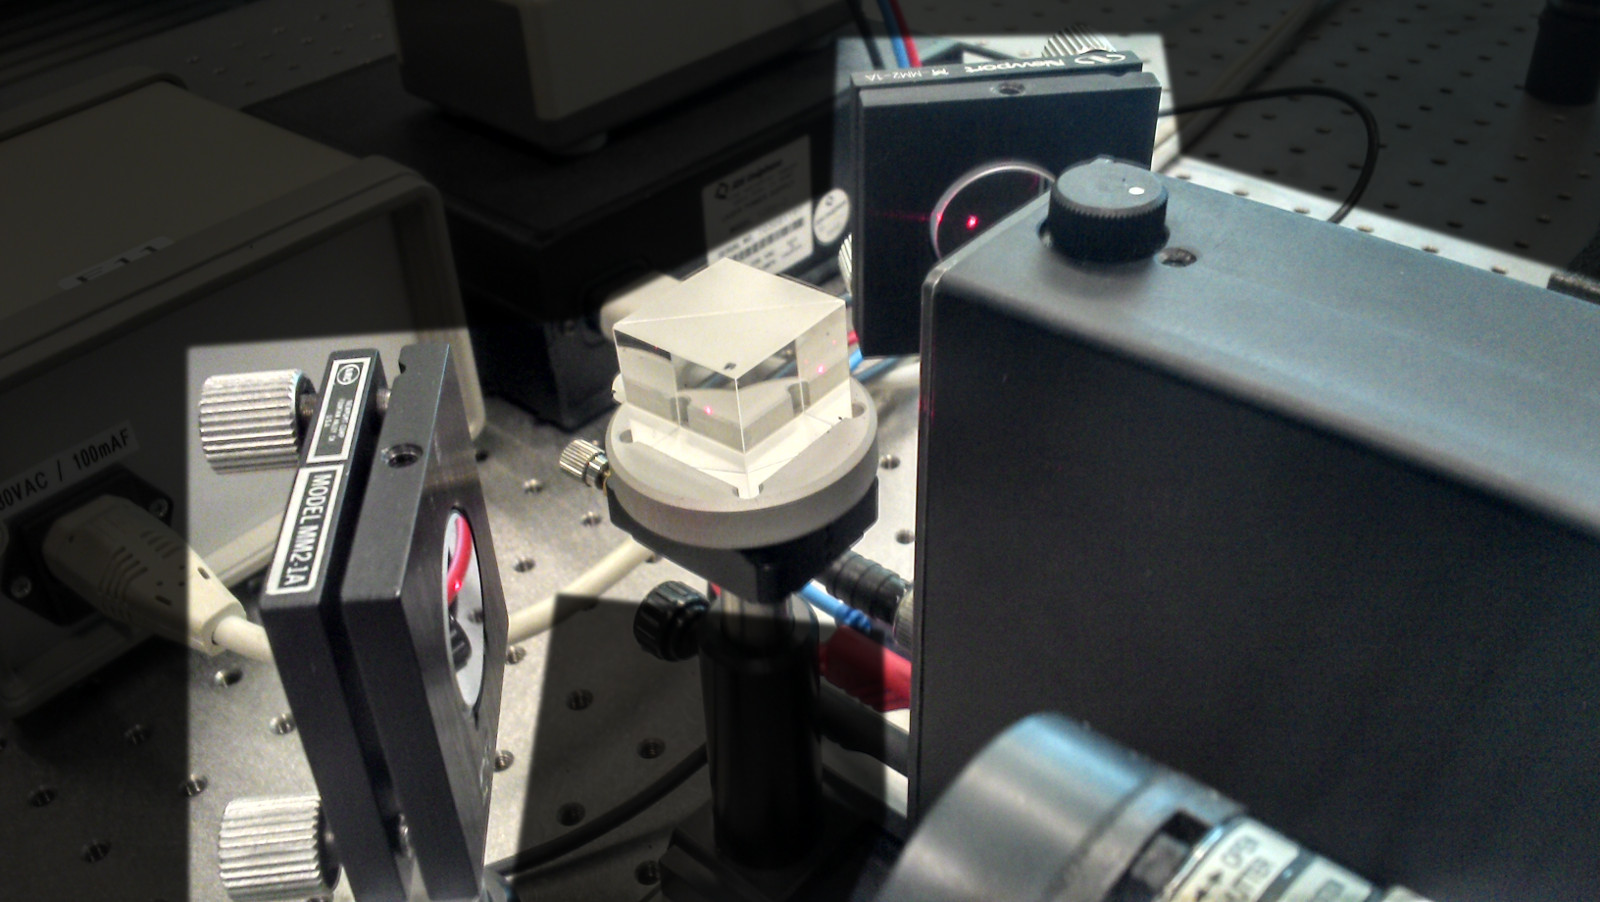
\includegraphics[width=.67\textwidth]{images/spiegel.jpeg}
    \caption{%
        Die beiden Spiegel und der Strahlteiler. Die Spiegel k\"onnen vestellt
        werden, um die Verl\"aufe der Strahlen aufeinander abzustimmen.
    }
    \label{fig:spiegel}
\end{figure}


\begin{figure}[h!t]
    \centering
    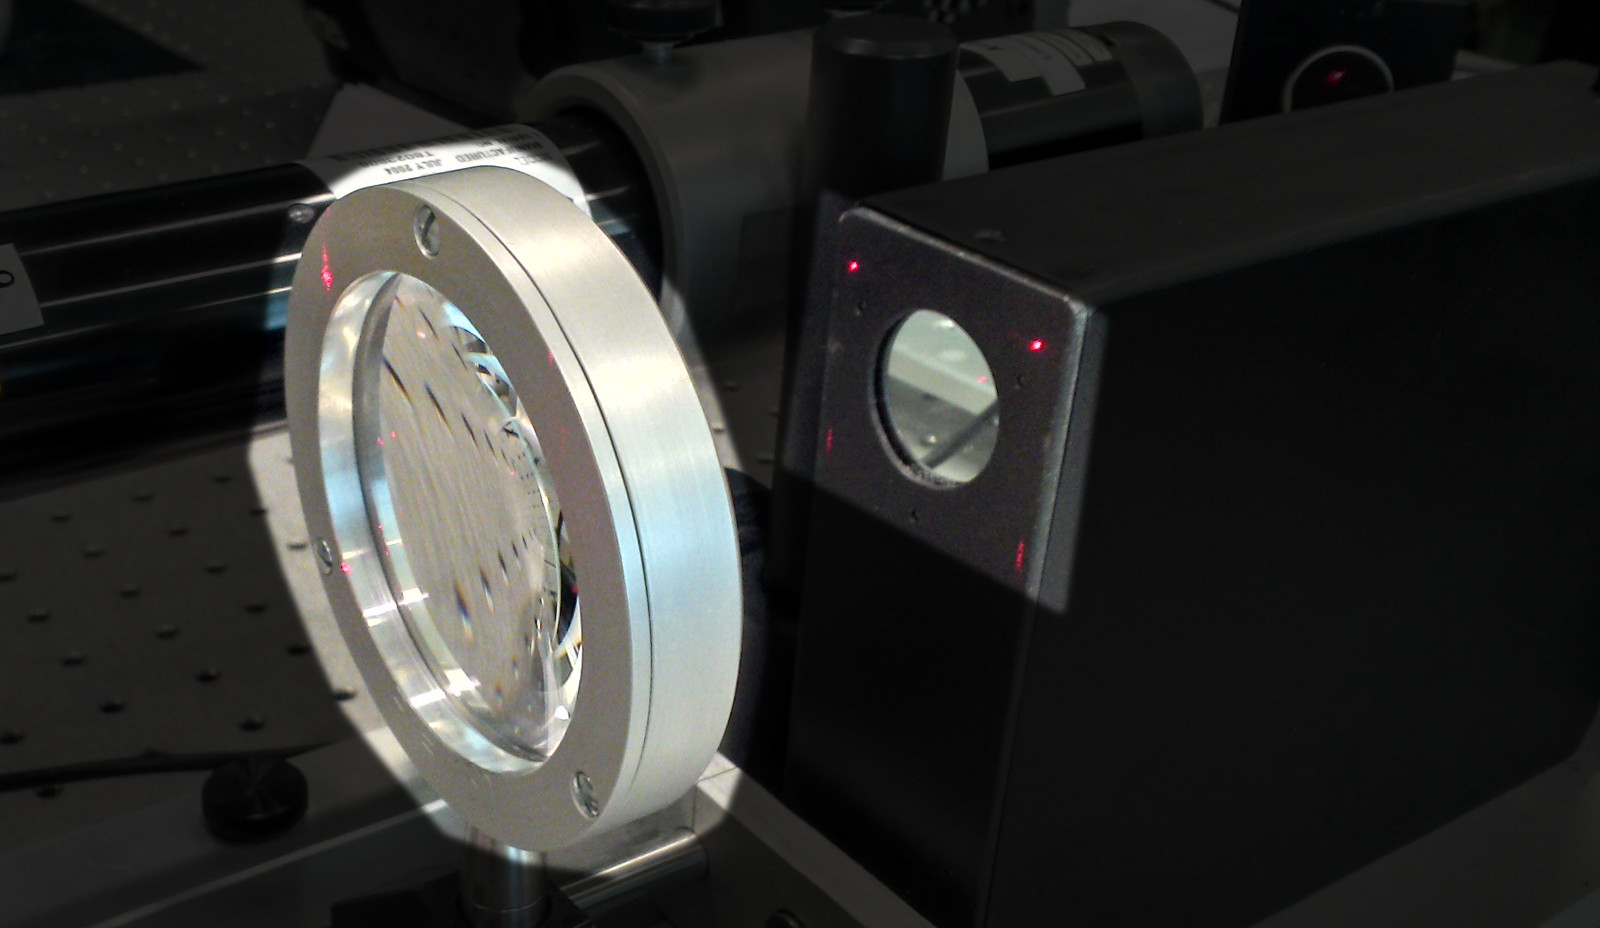
\includegraphics[width=.67\textwidth]{images/linse.jpeg}
    \caption{%
        Die  Linsen  $L_1$ (links,  gross)  und  $L_2$ (rechts,  im  schwarzen
        rechteckigen  Rahmen). Ebenfalls  sichtbar   sind  einige  Reflexionen
        der  Laserstrahlen am  Rahmen  von $L_2$,  bevor  sie justiert  worden
        sind. Nach der Justierung liegen alle vier Punkte auf gleicher H\"ohe.
    }
    \label{fig:lensL1}
\end{figure}

\begin{figure}[h!t]
    \centering
    \resizebox{.67\textwidth}{!}{\begin{tikzpicture}
    \begin{scope}[x={(0mm,300mm)},y={(0mm,199mm)},line width=1pt,cap=round]
        \node[anchor=south west,inner sep=0mm] at (0mm,0mm) {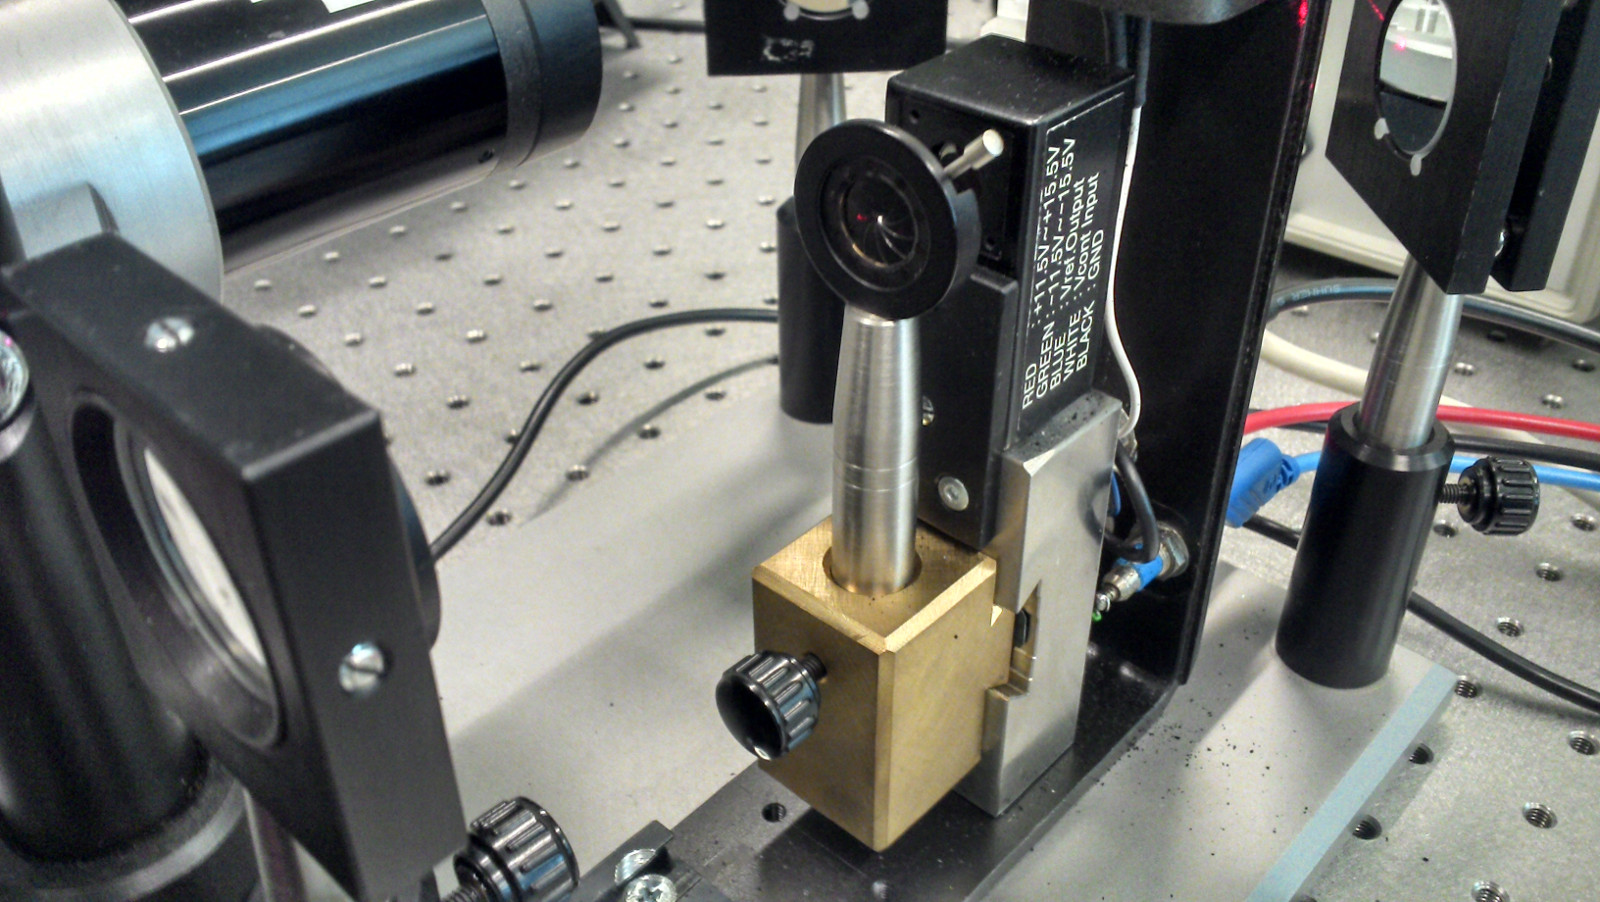
\includegraphics[width=300mm]{images/blende.jpeg}};

        %\draw[cyan] (210mm,80mm) -- (234mm,80mm);
        %\node[white] at (250mm,80mm) {\Large{\parbox{30mm}{\raggedright Geh\"ause mit \\Photomultiplier,\\ Blende und Linse $L_2$}}};
    \end{scope}
\end{tikzpicture}
}
    \caption{%
        Linse  $L_2$, Blende  und Photomultiplier. Die  Blende kann  verstellt
        werden,  um  m\"oglichst  nur  das  vom Str\"omungsteilchen  gestreute
        Laserlicht in den Photomultiplier zu lassen.
    }
    \label{fig:versuchsanordnung:blende}
\end{figure}

Die  Kreuzung  der   Laserstrahlen  in  der  Messleitung   kann  in  Abbildung
\ref{fig:laserkreuzung} gesehen werden.

\begin{figure}[h!t]
    \centering
    \resizebox{.67\textwidth}{!}{\begin{tikzpicture}
    \begin{scope}[x={(0mm,300mm)},y={(0mm,100mm)},line width=1pt,cap=round]
        \node[anchor=south west,inner sep=0mm] at (10mm,10mm) {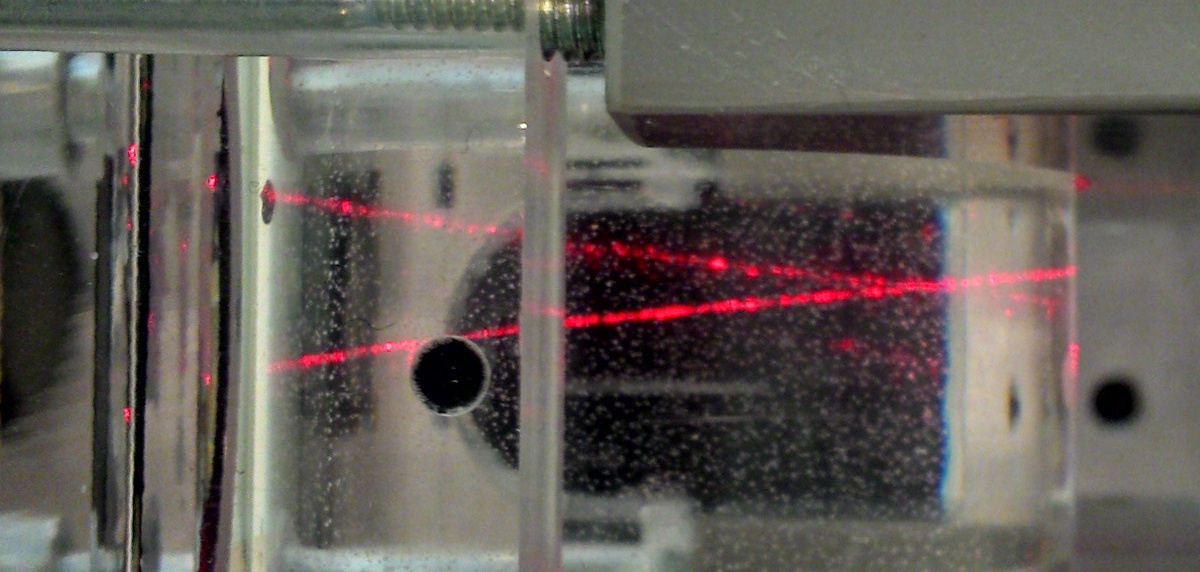
\includegraphics[width=260mm]{images/beams.jpeg}};

        \draw[-latex,line width=2pt] (5mm,30mm) -- (5mm,110mm);
        \node[rotate=90] at (1mm,65mm) {\huge{Wasserstr\"omung}};

        \draw[-latex,line width=2pt] (65mm,5.5mm) -- (230mm,5.5mm);
        \node at (150mm,0mm) {\huge{Einfallsrichtung Laserstrahlen}};
        %\draw[cyan] (210mm,80mm) -- (234mm,80mm);
        %\node[white] at (250mm,80mm) {\Large{\parbox{30mm}{\raggedright Geh\"ause mit \\Photomultiplier,\\ Blende und Linse $L_2$}}};
    \end{scope}
\end{tikzpicture}
}
    \caption{%
        Aufname      der     sich      kreuzenden     Strahlen      in     der
        Messleitung. Wasserstr\"omung   geht   von   unten  nach   oben,   die
        Laserstrahlen treffen von links auf die Messleitung.
    }
    \label{fig:laserkreuzung}
\end{figure}

Nachdem die Apparatur justiert war, wurden vier Messungen durchgef\"uhrt:

\begin{itemize}
    \item
        Eine experimentelle \"Uperpr\"ufung der Brennweite von Linse $L_1$,
    \item
        das  Verhalten  der  Str\"omungsgeschwindigkeit   auf  der  Achse  der
        Messleitung  bei Durchflussraten  zwischen \SI{0.5}{\liter\per\minute}
        und \SI{7.5}{\liter\per\minute},
    \item
        das  Geschwindigkeitsprofil   \"uber  den  gesamten   Querschnitt  der
        Messleitung bei \SI{0.5}{\liter\per\minute} (laminarer Fall) und
    \item
        das  Geschwindigkeitsprofil   \"uber  den  gesamten   Querschnitt  der
        Messleitung bei \SI{7.5}{\liter\per\minute} (turbulenter Fall).
\end{itemize}

Zur  Auswertung wurde  dabei das  Oszilloskop benutzt. Es  erhielt sowohl  das
ungefilterte Messsignal direkt from Photomultiplier (sehr verrauscht) wie auch
das gefilterte Signal aus dem Bandpassfilter.

Um  den  Bandpassfiter  korrekt  einstellen zu  k\"onnen,  musste  nat\"urlich
bekannt sein, in  welcher Gr\"ossenordnung sich die  zu erwartenden Frequenzen
ungef\"ahr befinden w\"urden.
%TODO: Frequency calculations

Das  Oszilloskop f\"uhrte  am  eingehenden  Zeitsignal eine  Fourier-Zerlegung
durch (unterstes Signal in Abbildung
% TODO: abbildung Oszi
).  In  diesem  Signal  wurden  dann mittels  der  beiden  Cursor  eine  obere
und  untere  Limite der  bei  einer  Einstellung (Position  des  Schnittpunkts
der  Laserstrahlen  in  der  Messleitung,  Flussgeschwindigkeit)  auftretenden
Frequenzen  abgelesen. Zur  Auswertung  wird  aus diesen  der  Mittelwert  mit
Unsicherheit gebildet (siehe Abschnitt.
%TODO Referenz
auf Seite
%TODO Referenz
).

Bei  \"andernden  Einstellungen musste  jeweils  darauf  geachtet werden,  den
Bandpass  entsprechend  anzupassen. Geht  dies   vergessen,  werden  zwar  die
Messresultate nicht  verf\"alscht, es  macht aber  das Erkennen  der gesuchten
Streu-Ereignisse zunehmend  schwierig oder verhindert sie  vollkommen, je nach
Frequenzbereich.


%TODO: Grunds\"atzlich: What happens when we do this? Might already have been explained
% in arbeitsgrundlagen.
